% https://tex.stackexchange.com/questions/750420/the-forbidden-nesting-of-matrices
\documentclass[tikz,border=1cm]{standalone}
\usepackage{nicematrix}
\usepackage{tikz}
\usetikzlibrary{matrix}
\NiceMatrixOptions{cell-space-limits = 5pt}
% https://tex.stackexchange.com/a/112212/322482
\makeatletter
\DeclareRobustCommand{\rvdots}{%
  \vbox{
    \baselineskip4\p@\lineskiplimit\z@
    \kern-\p@
    \hbox{.}\hbox{.}\hbox{.}
  }}
\makeatother
\newcommand*{\horizontalmatrix}{%
    \begin{bNiceMatrix}[first-row,margin]
            j=1 &  j=2 & \cdots & j=n-1 & j=n \\
            1  &  1  & \cdots &  1  &  1  \\
    \end{bNiceMatrix}
}
\newcommand*{\verticalmatrix}{%
    \begin{bNiceMatrix}[first-col,margin]
    j=1 & 0 \\
    j=2 & 1 \\
    \rvdots \hspace{1em}& \rvdots \\
    j=n-1 & 1 \\
    j=n & 1
    \end{bNiceMatrix}
}
\begin{document}
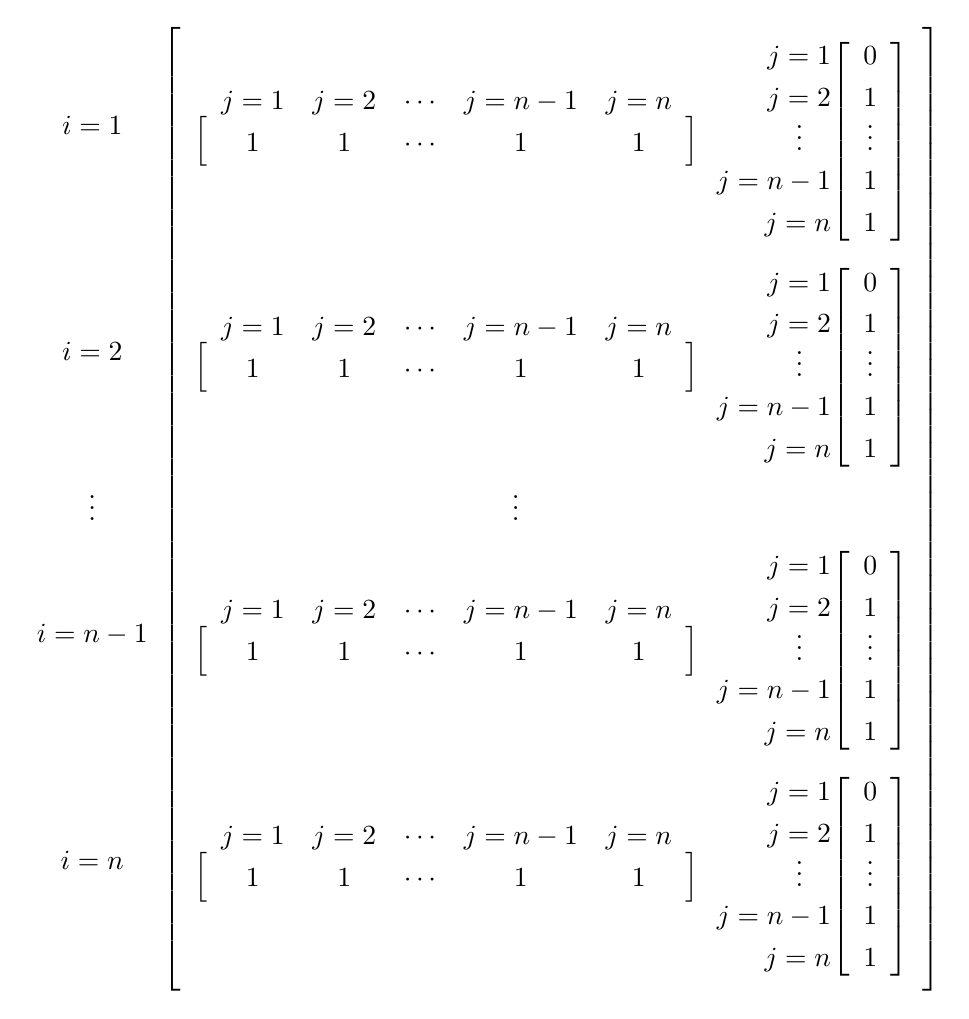
\begin{tikzpicture}
    \matrix (m) [%
        matrix of math nodes,%
        nodes={
            % draw=cyan,dashed,
            minimum size=.5cm,
            inner sep=0pt
        },
        row sep=1.5ex,column sep=1.5ex,
        left delimiter={[},right delimiter={]},
        ] {
        \horizontalmatrix & \verticalmatrix \\
        \horizontalmatrix & \verticalmatrix \\
        \hspace{5em}\rvdots  & \\
        \horizontalmatrix & \verticalmatrix \\
        \horizontalmatrix & \verticalmatrix \\
    };
    \foreach \i[count=\j] in {1,2,3,n-1,n}{
        \ifnum\j=3\relax
        \else
        \node at ([xshift=-4.5cm]m-\j-1) {$i=\i$};
        \fi
    }
    \node at ([xshift=-4.5cm]m-3-1) {$\rvdots$};
\end{tikzpicture}

\end{document}